	\section{Simulation model}
An accurate simulation of a quadrotor is a valuable asset, which allows safe and efficient development of control algorithms.
Additionally, it gives direct access to ground truth values and allows to design repeatable experiments.
The simulation environment selected is USARSim \cite{Balakirsky2009iros}, which is based on the Unreal Tournament game engine\footnote{\url{http://www.unrealengine.com/}}.
It allows physical realistic simulations and a versatile environment editor.

		\subsection{USARSim simulation environment}
		\subsection{Motion model}
The AR.Drone is a stabilized system (Figure \ref{fig:QuadRotorBody}). When no control signals are given the quadrotor hovers on the same location, which is accomplished by a feedback loop which uses the sonar (for altitude) and the bottom camera (for horizontal position). The simulation makes use of this assumption. When no control signal is given, the AR.Drone stays at the same location.
When a control signal for a longitudinal or lateral velocity is given, it calculates the force needed to reach that velocity (and assuming that the drag force $D_b$ increases linearly with the velocity). When the control signal stops, the drag force $D_b$ slows the quadrotor down until it hovers again.
The USARSim quadrotor model uses the Karma physics engine (part of the Unreal Engine \cite{Carpin2006}) to simulate the force and torque acting on the aircraft. Yet, only the overall thrust is calculated, the differential thrust is not used.
When moving in the horizontal plane, a real quadrotor changes its angle of attack (which is the defined as the angle between direction of motion $e_V$ and the body frame $e_N$ \cite{Yechout2003}). 
The Karma physics engine does not need this angle to calculate the resulting horizontal movement. Yet, this angle of attack has direct consequences for the viewing directions of the sensors, so the roll and the pitch should be adjusted in correspondence with horizontal movements. The active control of the AR.Drone is incorporated in the value of the dragforce $D_b$.

\begin{figure}[htb]
\centering
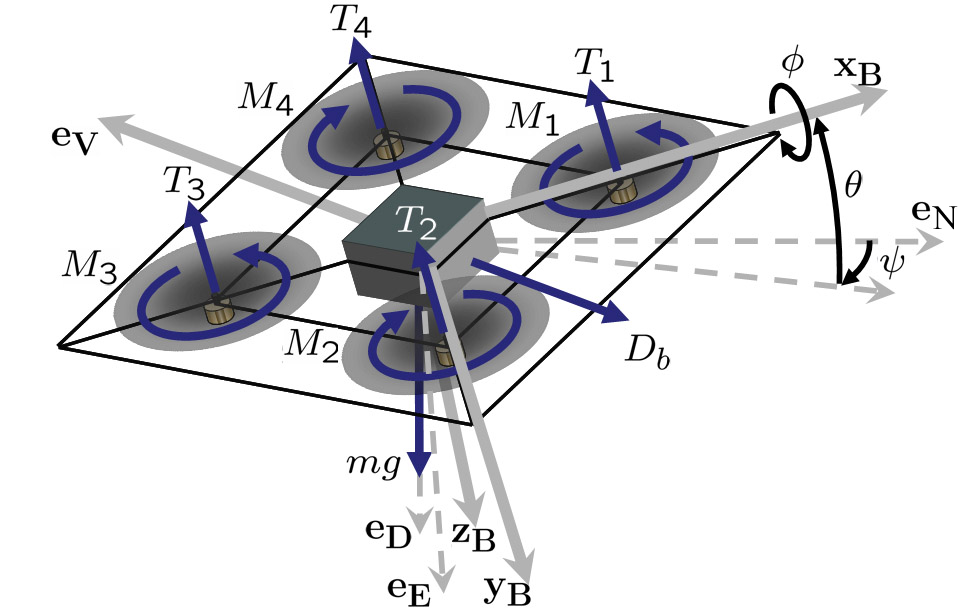
\includegraphics[width=7cm, height=5cm]{images/QuadRotorBody.png}
\caption{Free body diagram of a quadrotor helicopter 
%(Courtesy Hoffman \textit{et al.}
\cite{Hoffmann2007}. Note that a right-handed orthogonal coordinate system is used with the $z$-axis pointing down. Each of the 4 motors has a thrust $T_i$ and momentum $M_i$. Together the motors should generate sufficient vertical thrust to stay airborne, which is indicated by the gravity force $mg$ in the direction $e_D$. Differential thrust between the motors can provide roll $\phi$ and pitch  $\theta$ torques, which lead to an angle of attack $\alpha$. This can result in fast movements of the helicopter (e.g. in the horizontal plane) in the direction $e_V$ which a resulting drag force $D_b$. }
\label{fig:QuadRotorBody}
\end{figure}

Control signals for vertical and rotational movements (around the z-axis) are calculated in the same manner. For vertical movements not only the drag force $D_b$ is taken into account. In this case also the gravitational force $mg$ is included in the equation. Rotations around the z-axis stop quite quickly when no control signal is given. For this rotational movement a strong drag force $D_r = 20 \times D_b$ is used to model the additional inertia. 

\begin{figure}[htb!]
\centering
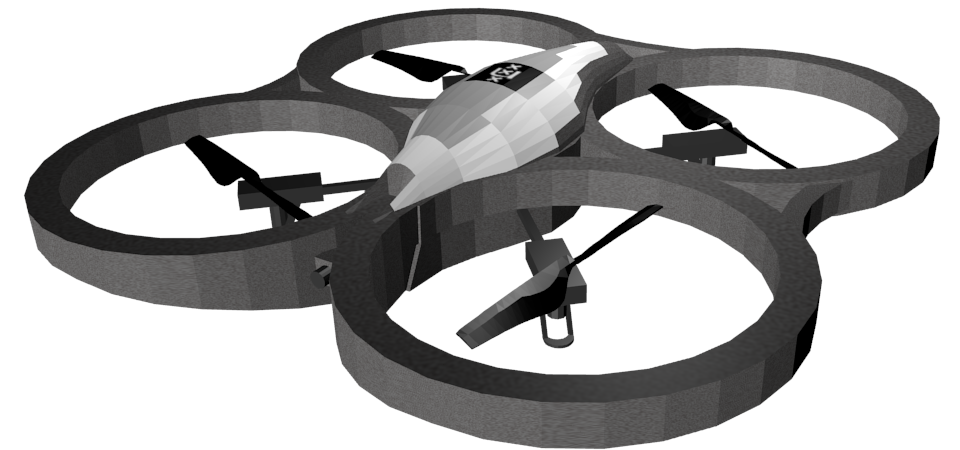
\includegraphics[width=6cm]{images/ardrone_blender_final.png}
\caption{3D model of the Parrot AR.Drone. This is a model optimized for simulation, based on the highly detailed model provided by Parrot SA.} 
\label{fig:3Dmodel}
\end{figure}

The result is a simulation model (Figure~\ref{fig:3Dmodel}), which maneuvers in a way similar to the actual AR.Drone, as demonstrated in Section~\ref{sec:validation_results}. Both the simulated and real system have the same dimensions $(0.525,0.515,0.115)\small{m}$. The principal elements of inertia are calculated correspondingly to $(0.0241, 0.0232, 0.0451)\small{kg\cdot m^2}$, assuming a homogeneous distribution of the mass.


		\subsection{Sensor model}
%Shortly describe your sonar model as implemented for USARSim and the camera-model (including natural lighting, shadows, resolution, white balance, etc).
The USARSim simulator has a set of configurable sensors, which include all the sensors from the AR.Drone.
Each mounted sensor is triggered at fixed time intervals (every $200\small{ms}$ by default).
The AR.Drone's time interval is reduced to $5\small{ms}$, producing up to 200 sensor measurements per second.

The sonar sensor emits a number of traces, which in combination form a cone.
First the sensor sends out one trace in the direction of its orientation remembering the measured range.
Then it does several conical measurements and calculates the minimal measured distance.
If the angle between a trace and the surface normal is smaller than angle $\alpha_{maxIncidence}$ the measurement is ignored.

The acceleration sensor computes the body accelerations using the AR.Drone's velocity:
\begin{equation}
a_{t} = (v_{t} - v_{t-\Delta t}) / \Delta t
\end{equation}
where $\Delta t$ is the time between measurements and $v$ is the velocity of the AR.Drone. The velocity of an object is modeled explicitly by the simulator.

The camera is modeled by creating a viewpoint in the Unreal engine.
%The sensors field of view property controls the camera's focal length.
The field of view is set to $64$ degrees and the resolution is set to $176 \times 144$ pixels, matching the specifications of the AR.Drone's bottom camera.
USARSim supports dynamic lightning to produce realistic images and shadows.
However, the camera sensor lacks a noise model and doesn't emulate the effect of automatic white balancing that is performed in most cameras (including the AR.Drone's camera).
Our previous paper \cite{Visser2011imav} briefly describes the influence of white balancing on image stitching and how to mimic the real images as close as possible.

\section{Proposed framework}
	\subsection{Abstracting from interfaces}